% !TeX encoding = UTF-8
% !TeX program = xelatex

\documentclass{YNUbachelor}
\usepackage{myPackages}

\title{云南大学本科学生毕业论文(设计)\;\LaTeX 模板}
\school{XX学院}
\author{XXX}
\studentID{20181050000}
\major{XX学}
\teacher{XXX}

\begin{document}
	
	\cover

	\copyrightpage
	
	\maketitle

	\toc

	\begin{abstract}
		中文摘要
	\end{abstract}

	\keywords{关键词1;关键词2;关键词3}

	\begin{enabstract}
		English Abstract
	\end{enabstract}

	\enkeywords{enKeyWords1;enKeyWords2;enKeyWords3}
		
	\section{基本使用说明}
		\subsection{编码与编译要求}
		\lstinline[language=latex]|main.tex|源代码必须保存为UTF-8编码,并使用XeLaLeX编译器进行编译,其在源代码中对应的语句为:
		
	\begin{latexcode}
		% !TeX encoding = UTF-8
		% !TeX program = xelatex
	\end{latexcode}
		
		注意:在\LaTeX 源代码中``\lstinline[language=latex]|%|''是注释符,但以上代码会指定相应的设置,因此在设置正确的前提下才能将其删去。另外,符号``\lstinline[language=latex]|\|''可以调用宏命令,形如\lstinline[language=latex]|\命令名[<可选参数>]{<必选参数>}|,也可以开启一个环境,形如\lstinline[language=latex]|\begin{<环境名>}[<可选参数>] ... \end{<环境名>}|,它还是一个转义符。这里使用符号\lstinline[language=latex]|< >|表示选项。
		
		\subsection{文档类和所需的宏包}
		通过如下命令导入文档类和所需的宏包:
	\begin{latexcode}
		\documentclass{YNUbachelor}
		\usepackage{myPackages}
	\end{latexcode}

	注意:为了使\lstinline[language=latex]|main.tex|源代码更加简洁,建议在\lstinline[language=latex]|myPackages.sty|文件中添加所需的宏包。
		
		\subsection{论文信息}
		将论文信息填在如下命令中:
	\begin{latexcode}
		\title{云南大学本科学生毕业论文(设计)\;\LaTeX 模板}
		\school{XX学院}
		\author{XXX}
		\studentID{20181050000}
		\major{XX学}
		\teacher{XXX}
	\end{latexcode}

	强烈建议将以上的这些代码写在\lstinline[language=latex]|main.tex|源代码靠前的位置。
	
	\section{撰写正文}
	\subsection{document环境}
	\lstinline[language=latex]|main.tex|文件中有且仅有一个\lstinline[language=latex]|document|环境,{\color{red}\bfseries 在此之后的所有代码}都必须写在\lstinline[language=latex]|document|环境中。
	\begin{latexcode}
		\begin{document}
			%此后的所有代码都必须写在这里
		\end{document}
	\end{latexcode}
	
	\subsection{论文封面、声明页、标题和目录}
	使用如下代码插入论文的封面、声明页、标题和目录:
	\begin{latexcode}
		\cover%论文封面
		
		\copyrightpage%声明页
		
		\maketitle%论文标题
		
		\toc%目录
	\end{latexcode}

	\subsection{中英文摘要及关键词}
	使用如下代码插入中英文摘要及关键词:
	\begin{latexcode}
		\begin{abstract}
			中文摘要
		\end{abstract}
		
		\keywords{关键词1;关键词2;关键词3}
		
		\begin{enabstract}
			English Abstract
		\end{enabstract}
		
		\enkeywords{enKeyWords1;enKeyWords2;enKeyWords3}
	\end{latexcode}
	
	\subsection{章节标题和段落}
	本模板中,一级标题、二级标题和三级标题分别使用\lstinline[language=latex]|\section{<一级标题名>}|、\lstinline[language=latex]|\subsection{<二级标题名>}|和\lstinline[language=latex]|\subsubsection{<三级标题名>}|表示。{\color{red}\bfseries 分段应空一行},换句话说:分段应按两次回车键,而不是一次。例如:
	
	\begin{latexcode}
		\section{一级标题名}
		这是第一段。
		
		这是第二段。
			\subsection{二级标题名}
			这是第一段。
			
			这是第二段。
				\subsubsection{三级标题名}
				这是第一段。
				
				这是第二段。
	\end{latexcode}
	
	\subsection{数学环境}
	
	在论文中排版数学符号、行内公式和行间公式是很方便的。对于初学者,推荐使用\href{https://www.latexlive.com/}{在线\LaTeX 公式编辑器}来辅助编辑\LaTeX 公式。以下介绍行内公式和行间公式的排版方式:
	\subsubsection{行内公式}
		行内公式应使用\lstinline[language=latex]|$ <公式的代码> $|来表示。例如:
	\begin{latexcode}
		勾股定理$a^2+b^2=c^2$。
	\end{latexcode}勾股定理$a^2+b^2=c^2$。

	\subsubsection{行间公式}
		行间公式应使用\lstinline[language=latex]|\[ <公式的代码> \]|来表示。例如:
	\begin{latexcode}
		勾股定理:
		\[
			a^2+b^2=c^2
		\]
	\end{latexcode}勾股定理:\[a^2+b^2=c^2\]
	
	\subsubsection{带有编号的行间公式}
		带有编号的行间公式应使用\lstinline[language=latex]|align|等环境来表示。例如:
		
	\begin{latexcode}
		勾股定理:
		\begin{align}
			a^2+b^2=c^2\label{eq:Pythagoras theorem}
		\end{align}
	\end{latexcode}
	勾股定理:\begin{align}
	a^2+b^2=c^2\label{eq:Pythagoras theorem}
	\end{align}

	\subsubsection{带编号公式的引用}
	上一小节中的\lstinline[language=latex]|\label{eq:Pythagoras theorem}|给公式一个标签,方便交叉引用。例如:
	
	\begin{latexcode}
		引用勾股定理,\autoref{eq:Pythagoras theorem}。
	\end{latexcode}引用勾股定理,\autoref{eq:Pythagoras theorem}。

	可以交叉引用的还有图片、表格和章节等,以下的内容会介绍。

	\subsection{插图}
	\subsubsection{插入图片的一般方式}
	\begin{latexcode}
		\begin{figure}[htbp]
			\centering
			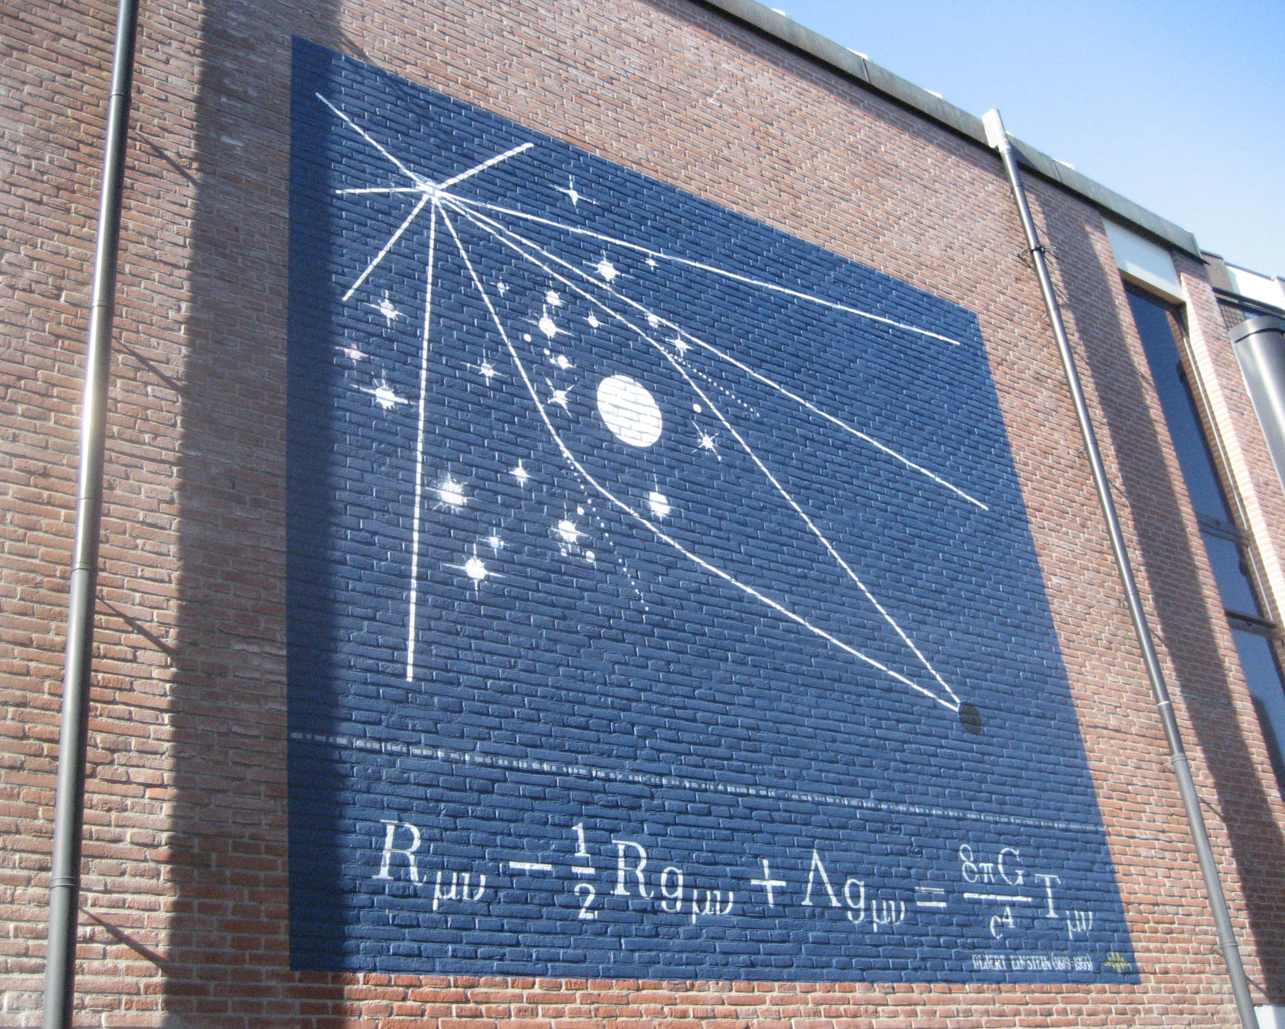
\includegraphics[width=0.7\linewidth]{fig}
			\caption{这是一个示例图片}
			\label{fig:一个示例图片}
		\end{figure}
	\end{latexcode}
		
	\subsubsection{使用TikZ绘图}
	\href{https://github.com/csekri/tkzgeom}{GUI tool for TikZ figure production}
	
	\begin{figure}[htbp]
		\centering
		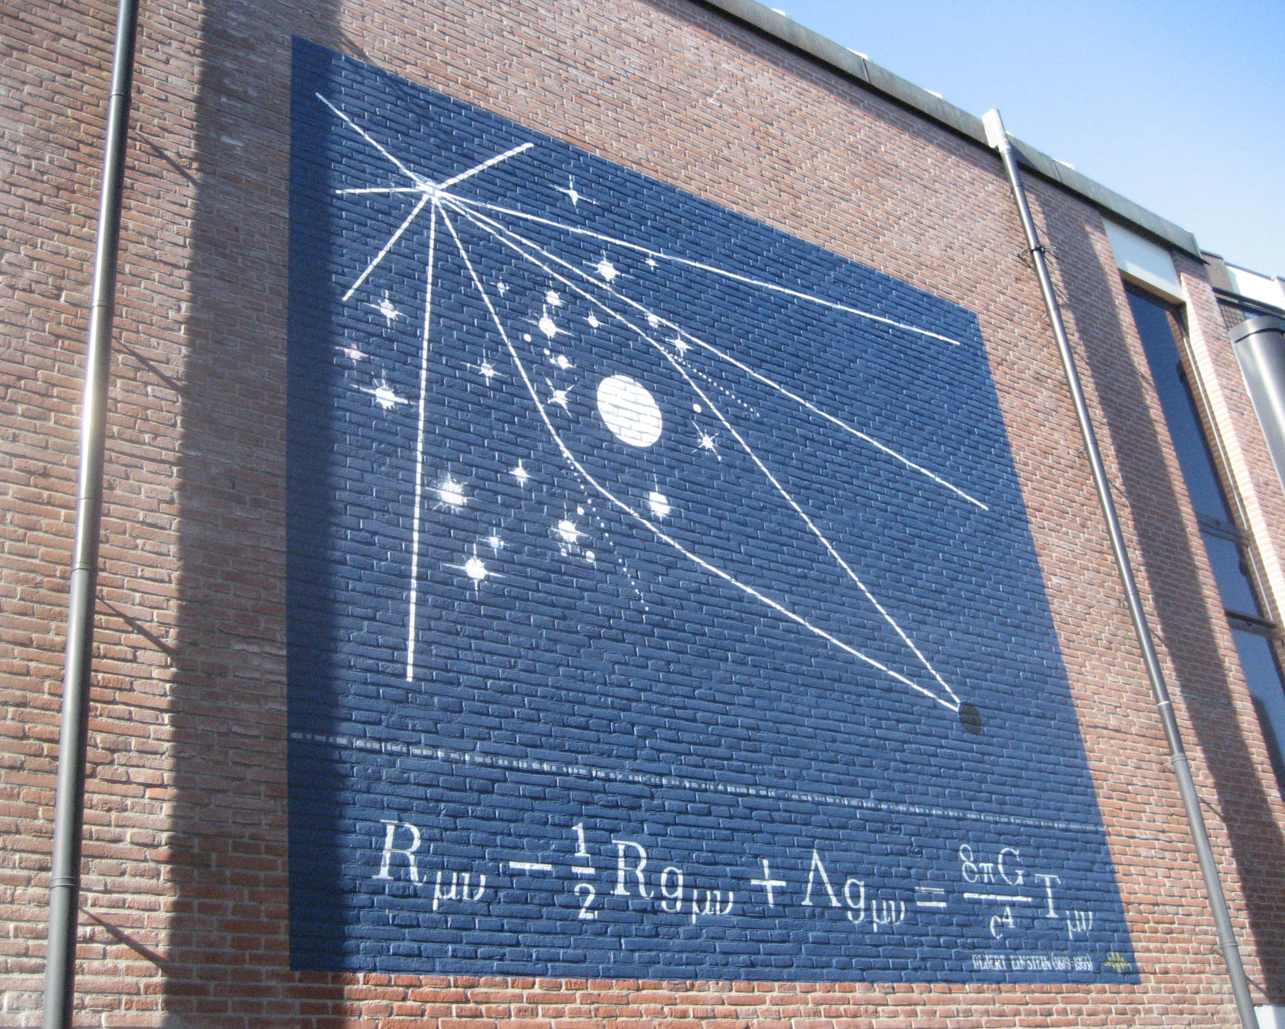
\includegraphics[width=0.7\linewidth]{fig}
		\caption{这是一个示例图片}
		\label{fig:一个示例图片}
	\end{figure}

	内容内容内容,引用图片\autoref{fig:一个示例图片}内容内容内容
	
	内容内容内容内容内容内容内容内容内容内容内容内容内容内容内容内容内容内容内容内容内容内容内容内容内容内容内容内容内容内容内容内容内容内容内容内容内容内容内容内容内容内容内容内容内容内容内容内容内容内容内容内容内容内。容内容内容内容内容内容内容内容内容内容内容内容内容内容内容内容内容内容内容内容内容内容内容内容内容内容内容内容内容内容内容内容内容内容内容内容内容内容内容。
	\subsection{画三线表}
	\href{https://tableconvert.com/}{表格在线转换}
	
	\begin{table}[htbp]
		\centering
		\caption{An example Table.}
		\label{tab:example}
		\begin{tabular}{lcc}
			\toprule
			Star & Mass & Luminosity\\
			& $M_{\odot}$ & $L_{\odot}$\\
			\midrule
			Sun & 1.00 & 1.00\\
			$\alpha$~Cen~A & 1.10 & 1.52\\
			$\epsilon$~Eri & 0.82 & 0.34\\
			\bottomrule
		\end{tabular}
	\end{table}
	\autoref{tab:example} 由如下代码生成:
	\begin{verbatim}
		\begin{table}[htbp]
			\centering
			\caption{An example Table.}
			\label{tab:example}
			\begin{tabular}{lcc}
				\toprule
				Star & Mass & Luminosity\\
				& $M_{\odot}$ & $L_{\odot}$\\
				\midrule
				Sun & 1.00 & 1.00\\
				$\alpha$~Cen~A & 1.10 & 1.52\\
				$\epsilon$~Eri & 0.82 & 0.34\\
				\bottomrule
			\end{tabular}
		\end{table}
	\end{verbatim}

	\subsection{代码片段}
	%\lstinputlisting[language=python,float=htbp]{code/Python example.py}
	
	\subsection{文献引用}
	引用\cite{向守平2008天体物理概论}。引用\cite{BQC_2020}。
	\begin{acknowledgement}
		致谢。
	\end{acknowledgement}

	\reference{references/references.bib}%参考文献,引入文献的bibtex格式信息,填bib文件路径
	
	%\lstinputlisting[language=latex,caption={\LaTeX~Source Code}]{main.tex}
	
	\backcover%封底
\end{document}
